\let\negmedspace\undefined
\let\negthickspace\undefined
\documentclass[journal,12pt,twocolumn]{IEEEtran}
\usepackage{cite}
\usepackage{amsmath,amssymb,amsfonts,amsthm}
\usepackage{algorithmic}
\usepackage{graphicx}
\usepackage{textcomp}
\usepackage{xcolor}
\usepackage{txfonts}
\usepackage{listings}
\usepackage{enumitem}
\usepackage{mathtools}
\usepackage{gensymb}
\usepackage{comment}
\usepackage[breaklinks=true]{hyperref}
\usepackage{tkz-euclide} 
\usepackage{listings}
\usepackage{gvv}                                        
\def\inputGnumericTable{}                                 
\usepackage[latin1]{inputenc}                                
\usepackage{color}                                            
\usepackage{array}                                            
\usepackage{longtable}                                       
\usepackage{calc}                                             
\usepackage{multirow}                                         
\usepackage{hhline}                                           
\usepackage{ifthen}                                           
\usepackage{lscape}
\newtheorem{theorem}{Theorem}[section]
\newtheorem{problem}{Problem}
\newtheorem{proposition}{Proposition}[section]
\newtheorem{lemma}{Lemma}[section]
\newtheorem{corollary}[theorem]{Corollary}
\newtheorem{example}{Example}[section]
\newtheorem{definition}[problem]{Definition}
\newcommand{\BEQA}{\begin{eqnarray}}
\newcommand{\EEQA}{\end{eqnarray}}
\newcommand{\define}{\stackrel{\triangle}{=}}
\theoremstyle{remark}
\newtheorem{rem}{Remark}
\begin{document}
\bibliographystyle{IEEEtran}
\vspace{3cm}
\title{11.9.4.4}
\author{EE23BTECH11027 - K RAHUL$^{*}$% <-this % stops a space
}
\maketitle
\newpage
\bigskip
\renewcommand{\thefigure}{\theenumi}
\renewcommand{\thetable}{\theenumi}
DERIVATIONS AND RESULTS: \\
\begin{align}
    x\brak{n} &= \frac{1}{n+c} u\brak{n},\text{where} \: c \in \mathbb{R}\\
    X\brak{z} &= \sum_{n= -\infty}^{n= +\infty} x\brak{n}z^{-n}\\
    &=\sum_{n = 0}^{n = +\infty} \frac{1}{n+c}z^{-n}\\
    &= z^c\sum_{n = 0}^{n = +\infty} \frac{1}{n+c}z^{-\brak{n+c}}\\
    &= z^c \biggl(-log\brak{1-z^{-1}}- z^{-1}-\frac{z^{-2}}{2}\notag \\& \;\;\;\;-\frac{z^{-3}}{3} - \ldots -\frac{z^{-(c-1)}}{c-1} \biggr)\label{11027_eq1}
\end{align} 
\begin{align}
    d\brak{z} &= z^{2}log\brak{1-z^{-1}}\\
    d\brak{n}&=\frac{1}{2\pi j} \oint _C z^{n+1}\log{\brak{1-z^{-1}}}dz\\
    &=\frac{-1}{2\pi j} \oint _C z^{n+1}\biggl(z^{-1}+\frac{z^{-2}}{2} + \frac{z^{-3}}{3}+\ldots + \frac{z^{-(n+1)}}{n+1} \notag\\ \;\: &+  \frac{z^{-\brak{n+2}}}{n+2}+ \ldots \biggr) dz\\
    &z=e^{jt}\\
    &=\frac{-1}{2\pi} \int_{0}^{2\pi} e^{\brak{n+2}jt}\biggl(e^{-jt}+\frac{e^{-2jt}}{2} + \frac{e^{-3jt}}{3} \notag \\&+.. +\frac{z^{-\brak{n+2}}jt}{n+2}+..\biggr) dz\\
    &=\frac{-1}{n+2}\label{11027_eq2}
\end{align}

\begin{align}
    d\brak{z}&= \frac{z^k}{1-z^{-1}},\text{where} \: k \in \mathbb{R}\\
    d\brak{n}&= \lim_{x \to 1}z^{n+k-1} \text{(Residue Theorem)}\\
    &= 1\label{11027_eq3}
\end{align}
\bigskip
QUESTION:\\
Find sum to n terms of the following series:\\
$\frac{1}{1 \times 2} + \frac{1}{2 \times 3} + \frac{1}{3 \times 4} + \ldots$
\bigskip \bigskip


SOLUTION:
\begin{table}[ht]
\setlength{\arrayrulewidth}{0.3mm}
\setlength{\tabcolsep}{15pt}
\renewcommand{\arraystretch}{1.5}



\begin{tabular}{ |p{1cm}|p{3cm}|p{1cm}| }
\hline
\multicolumn{3}{|c|}{Parameters in expression}\\
\hline
Symbol & Description & Value\\
\hline
$x(n)$ & $n^{th}$ term of series & \\
\hline
%$x(l)$ & Last($l^{th}$) term of series & 350\\
%$x(0)$ & Starting ($0^{th}$) term of series & 17 %\\
%\hline
%d & Common difference of AP & 9\\
%\hline
\end{tabular}
\caption{Parameters}
 %Table 1: Parameters


\end{table}
\begin{align}
x\brak{n} &= \frac{1}{\brak{n+1}\brak{n+2}}u\brak{n}\\
& = \brak{\frac{1}{n+1} - \frac{1}{n+2}}u\brak{n}\\
\end{align}
Using \eqref{11027_eq1}we get,
\begin{align}X\brak{z} &= -z log\brak{1-z^{-1}} + z^2 log\brak{1-z^{-1}} + z\\
&= z\brak{z-1}log\brak{1-z^{-1}} + z\\
    Y\brak{z} &= X\brak{z}U\brak{z}\\
     &=z^2log\brak{1-z^{-1}} + \frac{z}{1-z^{-1}} \\
\end{align}
\text{Using \eqref{11027_eq2} and \eqref{11027_eq3},}
\begin{align}
    y\brak{n} &= 1 - \frac{1}{n+2}
\end{align}
\begin{figure}[h]
    %\caption{Stem Plot of $x\brak{n}$ v/s n}
    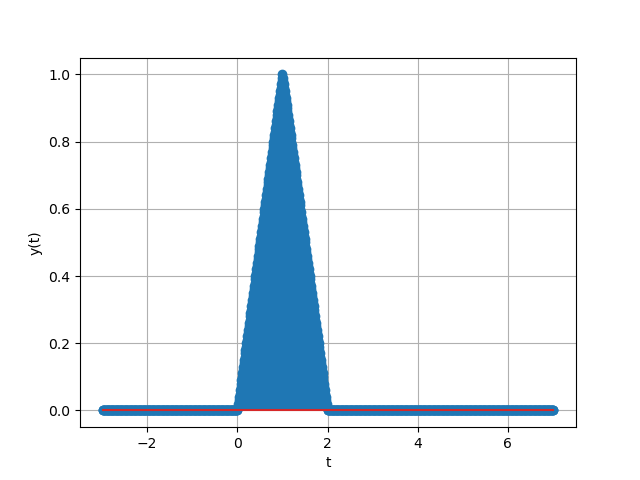
\includegraphics[width=0.3\textwidth]{figs/y(t)_vs_t.png}\label{fig:stem-plot}
    \caption{Stem Plot of $y\brak{t}$ v/s t}
\end{figure}
\end{document}


